%!TEX root=../GaugeCNNTheory.tex


\begin{subfigure}[b]{0.26\textwidth}
    \centering
    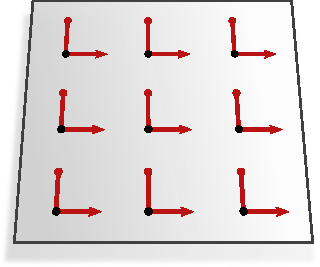
\includegraphics[width=1.\textwidth]{figures/G_structure_R2_1_big.pdf}
    \captionsetup{format=hang}
    \caption{\small
        \,  $M = \R^2$,
        \,\ $G = \{e\}$
    }
    \label{fig:G_structure_intro_a}
\end{subfigure}
\hfill
\begin{subfigure}[b]{0.26\textwidth}
    \centering
    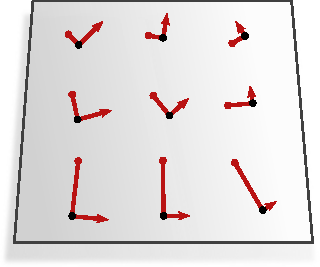
\includegraphics[width=1.\textwidth]{figures/G_structure_R2_5_big.pdf}
    \captionsetup{format=hang}
    \caption{\small
        \,  $M = \R^2$,
        \,\ $G = \{e\}$
    }
    \label{fig:G_structure_intro_b}
\end{subfigure}
\hfill
\begin{subfigure}[b]{0.26\textwidth}
    \centering
    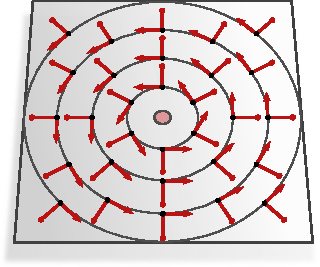
\includegraphics[width=1.\textwidth]{figures/G_structure_R2_no_origin_SO2_intro.pdf}
    \captionsetup{format=hang}
    \caption{\small
        \,  $M = \R^2\backslash\{0\}$,
        \,\ $G = \{e\}$
    }
    \label{fig:G_structure_intro_c}
\end{subfigure}
\\[2ex]
% 
% 
% 
% 
\begin{subfigure}[b]{0.26\textwidth}
    \centering
    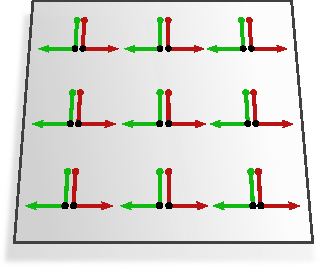
\includegraphics[width=1.\textwidth]{figures/G_structure_R2_3_big.pdf}
    \captionsetup{format=hang}
    \caption{\small
        \,  $M = \R^2$,
        \,\ $G = \Flip$
    }
    \label{fig:G_structure_intro_d}
\end{subfigure}
\hfill
\begin{subfigure}[b]{0.26\textwidth}
    \centering
    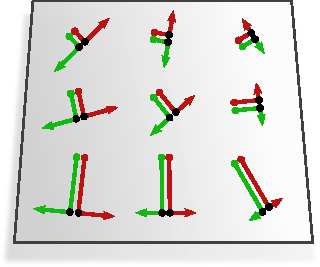
\includegraphics[width=1.\textwidth]{figures/G_structure_R2_6_big.pdf}
    \captionsetup{format=hang}
    \caption{\small
        \,  $M = \R^2$,
        \,\ $G = \Flip$
    }
    \label{fig:G_structure_intro_e}
\end{subfigure}
\hfill
\begin{subfigure}[b]{0.26\textwidth}
    \centering
    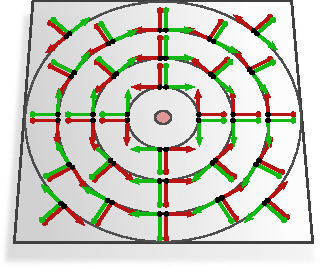
\includegraphics[width=1.\textwidth]{figures/G_structure_R2_no_origin_O2_intro.pdf}
    \captionsetup{format=hang}
    \caption{\small
        \,  $M = \R^2\backslash\{0\}$,
        \,\ $G = \Flip$
    }
    \label{fig:G_structure_intro_f}
\end{subfigure}
\\[2ex]
% 
% 
% 
% 
\begin{subfigure}[b]{0.26\textwidth}
    \centering
    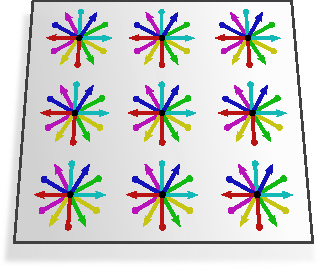
\includegraphics[width=1.\textwidth]{figures/G_structure_R2_2_big.pdf}
    \captionsetup{format=hang}
    \caption{\small
        \,  $M = \R^2$,
        \,\ $G = \SO2$
    }
    \label{fig:G_structure_intro_g}
\end{subfigure}
\hfill
\begin{subfigure}[b]{0.26\textwidth}
    \centering
    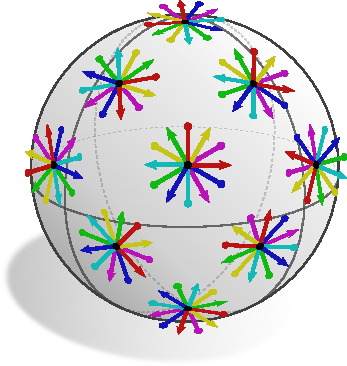
\includegraphics[width=.95\textwidth]{figures/G_structure_S2_1.pdf}
    \vspace*{-2ex}
    \captionsetup{format=hang}
    \caption{\small
        \,  $M = S^2$,
        \,\ $G = \SO2$
    }
    \label{fig:G_structure_intro_h}
\end{subfigure}
\hfill
\begin{subfigure}[b]{0.26\textwidth}
    \centering
    \makebox[\textwidth][c]{ % center over-wide figure
    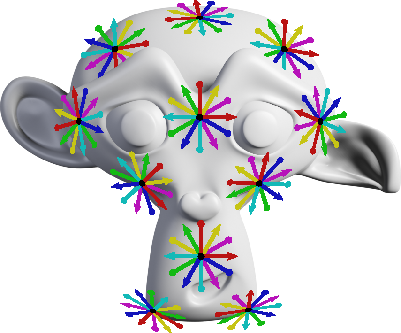
\includegraphics[width=1.12\textwidth]{figures/suzanne_SO2_structure.pdf}
    }
    \vspace*{-3.ex}
    \captionsetup{format=hang, width=1.1\textwidth}
    \caption{\small
        $M = \textup{``\href{https://en.wikipedia.org/wiki/Blender_(software)\#Suzanne}{Suzanne}''}$\!,
        \ $G = \SO2$
    }
    \label{fig:G_structure_intro_i}
\end{subfigure}
\\[2ex]
% 
% 
% 
% 
\begin{subfigure}[b]{0.26\textwidth}
    \centering
    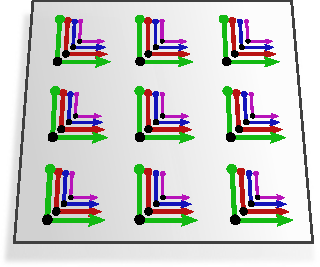
\includegraphics[width=1.\textwidth]{figures/G_structure_R2_4_big.pdf}
    \captionsetup{format=hang}
    \caption{\small
        \,  $M = \R^2$,
        \,\ $G = \Scale$
    }
    \label{fig:G_structure_intro_j}
\end{subfigure}
\hfill
\begin{subfigure}[b]{0.26\textwidth}
    \centering
    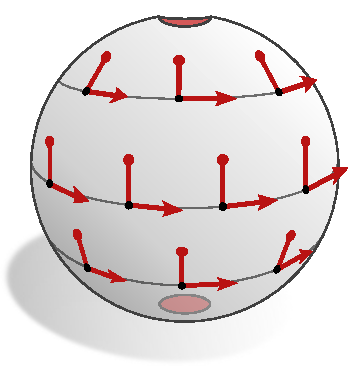
\includegraphics[width=.95\textwidth]{figures/G_structure_S2_2.pdf}
    \vspace*{-2ex}
    \captionsetup{format=hang}
    \caption{\small
        \,  $M = S^2\backslash$poles,
        \,\ $G = \{e\}$
   }
    \label{fig:G_structure_intro_k}
\end{subfigure}
\hfill
\begin{subfigure}[b]{0.26\textwidth}
    \centering
    \makebox[\textwidth][c]{ % center over-wide figure
    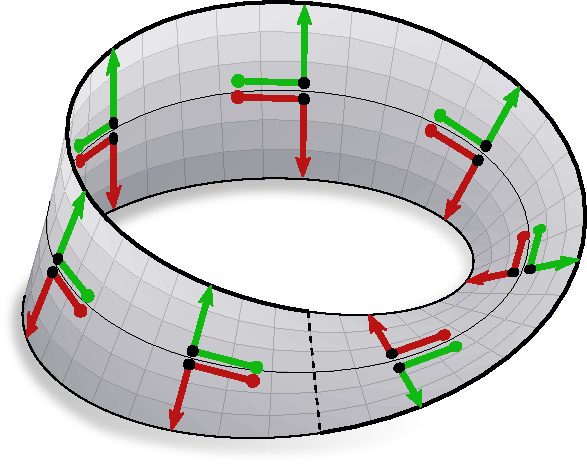
\includegraphics[width=1.1\textwidth]{figures/Mobius_R_structure.pdf}
    }
    \vspace*{-3.ex}
    \captionsetup{format=hang}
    \caption{\small
        \,  $M = \textup{M\"obius}$,
        \,\ $G = \Flip$
    }
    \label{fig:G_structure_intro_l}
\end{subfigure}
